\documentclass[12pt,letterpaper]{article}
\usepackage{graphicx,textcomp}
\usepackage{natbib}
\usepackage{setspace}
\usepackage{fullpage}
\usepackage{color}
\usepackage[reqno]{amsmath}
\usepackage{amsthm}
\usepackage{fancyvrb}
\usepackage{amssymb,enumerate}
\usepackage[all]{xy}
\usepackage{endnotes}
\usepackage{lscape}
\newtheorem{com}{Comment}
\usepackage{float}
\usepackage{hyperref}
\newtheorem{lem} {Lemma}
\newtheorem{prop}{Proposition}
\newtheorem{thm}{Theorem}
\newtheorem{defn}{Definition}
\newtheorem{cor}{Corollary}
\newtheorem{obs}{Observation}
\usepackage[compact]{titlesec}
\usepackage{dcolumn}
\usepackage{tikz}
\usetikzlibrary{arrows}
\usepackage{multirow}
\usepackage{xcolor}
\newcolumntype{.}{D{.}{.}{-1}}
\newcolumntype{d}[1]{D{.}{.}{#1}}
\definecolor{light-gray}{gray}{0.65}
\usepackage{url}
\usepackage{listings}
\usepackage{color}
\usepackage{verbatim} % includes comment blocks
%\usepackage[utf8]{inputenc}
%\usepackage{cancel}
%\usepackage{upquote}
\usepackage{amsmath}

\definecolor{codegreen}{rgb}{0,0.6,0}
\definecolor{codegray}{rgb}{0.5,0.5,0.5}
\definecolor{codepurple}{rgb}{0.58,0,0.82}
\definecolor{backcolour}{rgb}{0.95,0.95,0.92}

\lstdefinestyle{mystyle}{
	backgroundcolor=\color{backcolour},   
	commentstyle=\color{codegreen},
	keywordstyle=\color{magenta},
	numberstyle=\tiny\color{codegray},
	stringstyle=\color{codepurple},
	basicstyle=\footnotesize,
	breakatwhitespace=false,         
	breaklines=true,                 
	captionpos=b,                    
	keepspaces=true,                 
	numbers=left,                    
	numbersep=5pt,                  
	showspaces=false,                
	showstringspaces=false,
	showtabs=false,                  
	tabsize=2
}
\lstset{style=mystyle}
\newcommand{\Sref}[1]{Section~\ref{#1}}
\newtheorem{hyp}{Hypothesis}


\title{Applied Stats I: Exam 2}
\date{Due: December 9, 2022}
\author{Imelda Finn, 22334657}


\begin{document}
	\maketitle

	\section*{Instructions}
	Please read carefully: You have from 09:00 Wednesday December 7 until 08:59
Friday December 9 to complete the exam. Please export your answers as a single
PDF file and include all code you produce in a supporting R file, which you will
upload to Blackboard. The exam is open book; you can consult any materials you
like. You must not collborate with or seek help from other students. In case
of questions or technical difficulties, you can contact Professor Ziegler via email. You
should write-up your answers in R and LaTeX as you would for a problem set. Please
make sure to concisely number your answers so that they can be matched with the
corresponding questions.

\section*{Question 1}
\noindent  This data set presents information on 33 lambs, of which 11 are ewe lambs, 11 are wether
lambs, and 11 are ram lambs. These lambs grazed together in the same pasture and were
treated similarly in all ways. The variables of interest are presented in the table below.

\begin{table}[!htbp]
	\centering 
	\textbf{Table 1: Outcome and predictors for model.}\\
	\begin{tabular}{@{\extracolsep{5pt}}lc} 
	  Variable & Description \\ 
		\hline \\
	  Fatness & Continuous measure of leanness \\
	  Weight & Weight of lamb (kg) \\
	  Group  & Factor (ewe, wether, ram)\\
		\hline \\
	\end{tabular}\\
\end{table}


The objective is to determine whether differences in Fatness could be attributed to Group
while accounting for Weight. Information on the data and the model fit in R are given below:
\begin{verbatim}
  > names(lambs)
  [1] "Fatness" "Weight" "Group"
  
  > n = 33
  > Group.dummy.1 = rep(0,n)
  > Group.dummy.1[Group=="Wether"]=1
  > Group.dummy.2 = rep(0,n)
  > Group.dummy.2[Group=="Ram"]=1
  
  > lm.out= lm(Fatness ~ Weight + Group.dummy.1 + Group.dummy.2)
  > summary(lm.out)
  

Coefficients:
                        Estimate Std. Error t value Pr(>|t|)    
 (Intercept)         -18.1368  3.5213   -5.151 1.67e-05 ***
  Weight               2.2980  0.2248   10.223 3.99e-11 ***
  Group.dummy.1        -8.3622  0.9641   -8.674 1.50e-09 ***
  Group.dummy.2        -4.0716  0.9045   -4.502 0.000101 ***
  ---
  Signif. codes:  0 `***' 0.001 `**' 0.01 `*' 0.05 `.' 0.1 ` ' 1

Residual standard error: 2.012 on 29 degrees of freedom
Multiple R-squared:  0.8206,	Adjusted R-squared:  0.8021 
F-statistic: 44.23 on 3 and 29 DF,  p-value: < 6.075e-11

\end{verbatim} 

\begin{enumerate}[a)]
  \item Write out the fitted model for a wether lamb using the estimated coefficients.
  
  The general model is:
  \begin{gather}
    \beta_0 = -18.1368, \beta_{weight} = 2.2980, \delta_{wether} = -8.3622, \delta_{ram} = -4.0716,\notag\\
    \widehat{Fatness} = \beta_0 + Weight\beta_{weight} + Group.dummy.1\times\delta_{wether} + Group.dummy.2\times\delta_{ram} \label{eq:fat}
  \end{gather}

  For a wether lamb, $Group.dummy.1$ = 1 and $Group.dummy.2$ = 0, so  
  \[\widehat{Fatness} = \beta_0 + Weight\beta_{weight} + 1\times\delta_{wether} + 0\]
  
  
  so, the $Fatness$ of a wether lamb is predicted to be 
  \[-18.1368 + Weight\times 2.2980 - 8.3622 = -26.499 +  Weight\times 2.2980\]
  
  \item What is the predicted Fatness index of a ram lamb that weighs 10kg?
  
  from~\eqref{eq:fat}:
   \[\widehat{Fatness} = \beta_0 + Weight\beta_{weight} + 0 + 1\times\delta_{ram} \]
   \[ = -18.1368 + 10\times 2.2980 + (-4.0716) = 0.7716\] 
  
 
  \item Which lamb group has the highest Fatness index for every weight?
  
  The coefficients for wether and ram are both negative, so at any weight a ewe lamb will have the highest fatness index.

\end{enumerate}

\newpage

\section*{Question 2}
  \noindent Please select the most appropriate option to correctly answer each question.
Which of the following plots is used to check for normality in the assumptions of linear
regression?
%For quantitative variables, the most common assumption is that the conditional distribution of y is normal at each fixed value of x., AF 266
  \begin{enumerate}
    \item \textcolor{gray}{Scatterplot between residuals and X}
    \item \textcolor{gray}{Scatterplot between residuals and Y}
    \item \textcolor{gray}{Histogram of Y}
    \item \textbf{QQ plot of residuals}
  \end{enumerate}

  \noindent For explanatory variables with multi-collinearity, the corresponding estimated slopes have %$_________$
  \ldots standard errors.
  \begin{enumerate}
    \item \textbf{Larger}
    \item \textcolor{gray}{Smaller}
    \item \textcolor{gray}{The same}
  \end{enumerate}


  \noindent We can calculate our standard errors by taking the square root of the off-diagonal elements in our variance-covariance matrix.
  \begin{enumerate}
    \item \textcolor{gray}{True}
    \item \textbf{False}
  \end{enumerate}

  \noindent The coefficients in an ordinary least squares regression model \ldots.
  \begin{enumerate}
    \item \textcolor{gray}{are generalized additive estimates}
    \item \textcolor{gray}{are maximum likelihood estimates}
    \item \textbf{minimize the residual sum of squares}
    \item \textcolor{gray}{maximize the regression sum of squares}
  \end{enumerate}

\newpage

\section*{Question 3}
\noindent  Define and describe why the following four (4) terms are important to hypothesis testing
and/or regression. You can earn full credit with just two or three sentences, but please be
specific and thorough.
  \begin{enumerate}[(a)]
    \item \textbf{Partial F-test}
    
    An overall F-test tests whether all the regression coefficients in a model are $= 0$, ie whether any of the predictors are useful.  
    
    In order to test whether a subset of the coefficients are $= 0$, we use a partial F-test.  This tests the hypothesis that, in a model with $k$ coefficients:
    
    \(H_0 : \beta_1 = \beta_2 = ... = \beta_{p}, p < k\)
    vs \(H_a : \beta_i\), for some $i$, in $(1,p)$
    
    \[ F = \frac{\frac{RegSS_{reduced} - RegSS_{full}}{p}}{\frac{RSS_{full}}{n-k-1}} \]

which has a central F-distribution with numerator df $p$ (\# variables we are subsetting) and denominator df $n-k-1$.  The numerator is a measure of the increase in standard error that comes from using the partial model rather than the full one.

    We are testing whether the partial effect of several predictors as a group are significant in explaining the outcome variable, given the other variables in the model, for example we might want to test the significance of a multiplicative model, with the interactive term(s) excluded.

    \item \textbf{Constituent term}
    
    In an interactive regression model, the coefficients for the independent variables do not represent a constant effect of the independent variable on the dependent variable.  Each coefficient represents part of the effect of the dependent variables on the independent variable, and each dependent variable can constitute part of the multiplicative term(s).  If the model is 
    $y = \beta_0 + x\beta_1 + d\beta2+ \overbrace{dx}^m\beta_3$,
    then d and x are constitutent terms of term $m$.\footnote{https://www.yumpu.com/en/document/read/38069167/dummy-variables-and-multiplicative-regression-department-of-}
    
    \item \textbf{Test statistic}
    
    Test statistics are used in hypothesis testing.  The test statistic
summarizes how far that estimate falls from the parameter value under our null hypothesis ($H_0$). Often this is expressed by the number of standard errors between the estimate and the $H_0$ prediction.  
  If $H_0$ is true, we expect our observed value to match our predicted value.  The difference between these values is standardised and then compared to an appropriate probability distribution.  A higher absolute value of the test statistic means a lower probability that observed value is consistent with our null hypothesis.
  
  The test statistic will follow a probability distribution, under the null hypothesis, and this distribution can be used to find the probability that we would observe the values in our data, if $H_0$ is true.
  
  For example, to test whether an independent variable is a statistically reliable predictor of a dependent variable in a bivariate linear model $(y=\alpha + \beta x)$, we calculate a test statistic:
  
  \[t = \frac{\beta - 0}{se_{\beta}} \]
  
  $\beta$ is the observed value, 0 is our predicted value, given a null hypothesis that the variable is not a predictor.  This test statistic follows the Student's t-distribution, with degrees of freedom equal to the number of observed values, less the number of estimated coefficients.  The probability associated with the test statistic can then be compared to the pre-defined $\alpha$ value.  If the probability is less than our threshhold, we can reject the null hypothesis at that level of probability.

  
    \item \textbf{Residuals}
    
    We define a residual to be the observed value minus the predicted value.  For a  bivariate linear model our prediction is: $(\hat{y}=\alpha + \beta x)$; the residual value is $\epsilon = y - \hat{y}$.  For a multivariate model, the residual is the distance from a plane.
    
    A better model has lower absolute residuals, ie smaller distances between the predicted line and the observations.  The linear model assumes that the residuals are normally distrbuted around the regression line and have mean 0 and constant variance for all values of $x$.  A least squares model aims to minimise the sum of the squares of the residuals.  The residuals are used to calculate the estimate for $\sigma^2$, which is used in hypothesis testing pf the model coefficients.
    
    Analysing residuals can give us information about the quality of our model (eg allow us to check normality and constant variance assumptions), and can allow us to control for some variables so that we can get a clear view of the relationship between others.  We can also use them to calculate an estimate of the variation in our dependent variable which is accounted for by our model ($R^2$).
    
    
    
    
  \end{enumerate}


\newpage
\section*{Question 4}
\noindent Many of the wells used for drinking water in Bangladesh and other South Asian countries are contaminated with natural arsenic, affecting an estimated 100 million people. Arsenic is a
cumulative poison, and exposure increases the risk of cancer and other diseases, with risks
estimated to be proportional to exposure.

We performed a regression analysis with the data to understand the factors that predict
the arsenic level of 1000 households' drinking water. Your outcome variable $arsenic$ is a
continuous measure of household $i$'s arsenic level in units of hundreds of micrograms per liter.

We estimated models with the following inputs:
  \begin{itemize}
    \item The distance (in kilometers/100) to the closest known commercial factory
    \item Depth of respondent's well (binary variable; deep=1, not deep=0)
  \end{itemize}

  \begin{enumerate}[(a)]
    \item \textcolor{gray}{First, we successfully estimated an additive model with well depth and distance to
the nearest factory as the two predictors of a household's arsenic level. The estimated
coefficients are found in the first column of the table above. Interpret the estimated
coefficients for the intercept and each predictor.}

    With zero distance to the nearest factory and a shallow well, the arsenic is predicted to be -0.03 hundred micrograms per liter.
    
    Each unit increase in distance from the nearest factory of (in kilometers/100), decreases the arsenic level by 4.62 hundred micrograms per liter (for a given well depth).  This is statistically reliable at $\alpha = 0.01$.
    
    A household with a deep well will have an increased arsenic level of 3.33 hundred micrograms per liter, compared to one with a shallow well, assuming a constant distance from the nearest factory.

    \item \textcolor{gray}{Does the coefficient estimate for the closest known factory vary based on whether or not
a house has a deep well? If so, change your interpretation of the estimated coefficients
in part (a) to conform with the interactive model in column 2 of the table above. What
is the appropriate test to determine whether we should model the relationship between
distance, well depth, and arsenic levels using an additive or interactive model? What
information would you need to perform that test?}

    Model 1 is an additive model, the two predictors are assumed to be independent and therefore a change in value for $well.depth$ does not alter the coefficient for $dist100$.  In Model 2, there is an interaction assumed, which means the coefficient for the distance to the closest known factory changes from $-0.06$, with $well.depth=0$ to $-4.56$ when $well.depth=1$.  
    
    With zero distance to the nearest factory and a shallow well, the arsenic is predicted to be $-5.73$ hundred micrograms per liter.
    
    Each unit increase in distance from the nearest factory of (in kilometers/100), decreases the arsenic level by 0.06 hundred micrograms per liter with a shallow well, and by 4.56 hundred micrograms per liter with a deep well. 
    
    A household at a given distance from the nearest factory with a deep well will have a difference in arsenic level of $ + 8.95 - 0.06 \times dist100$ units, compared to one with a shallow well at the same distance.
 This is significant at $\alpha = 0.1$.
    
    If the coefficient for the interaction term is 0, we conclude that interaction is not significant, and we would prefer the additive model.  We can use a hypothesis test to check whether the interaction in this case is relevant, ie whether the coefficient for the multiplicative term is statistically reliable.  Assuming $\alpha = 0.05$
    
    \begin{align*}
      H_0: & \beta_{mult} = 0\\
      H_a: & \beta_{mult} \ne 0\\
      tstat = & \beta{mult} / se_{mult} = -4.50 / 2.66 = -1.691729\\
      p(>|t_{996}|) = & 0.0910104  
    \end{align*}
    
    Our p-value is not less than $\alpha$, so we cannot reject the null hypothesis.
    We are not confident that the interactive term is statistically relevant/reliable.
    
	 \lstinputlisting[language=R, firstline=74, lastline=83]{exam_22334657_ImeldaFinn.R}


    \item \textcolor{gray}{Using the `preferred' model from Part B, compute the average difference in arsenic
levels between two households that have a deep well (=1), but one is closer to a factory
(dist100 = 0.4) than the other (dist100 = 2.08).  }
    
    As the hypothesis test in (c) did not rule out the null hypothesis, we prefer the simpler, additive, model.\footnote{The $R^2$ for the additive model is 0.14, and for the interactive model is 0.15, which is not enough to make model 2 more attractive.}
    
    Household a: $well.depth = 1, dist100 = 0.04$
 
    $\widehat{arsenic_a} = -0.03 + 3.33 \times 1 + (-4.62) \times 0.04 = 1.452$
 
    Household b: $well.depth = 1, dist100 = 2.08$
 
    $\widehat{arsenic_b} = -0.03 + 3.33 \times 1 + (-4.62) \times 2.08 = -6.3096$
    
    average difference in $arsenic = 1.452 - (-6.3096) = 7.7616$ hundred micrograms per liter

	 \lstinputlisting[language=R, firstline=85, lastline=88]{exam_22334657_ImeldaFinn.R}

  \end{enumerate}


\begin{comment}
Model 1 Model 2
(Intercept) −0.03 (2.26) −5.73 (4.06)
well_depth 3.33 (2.14) 8.95 (3.95)
dist100 −4.62 (0.36) −0.06 (2.72)
well_depth:dist100 −4.50 (2.66)
R2 0.14 0.15
Adj. R2 0.14 0.14
Num Obs. 1000 1000
\end{comment}

\begin{table}[!htbp]
	\centering 
	\textbf{Table 2: Estimated coefficients from regression predicting arsenic levels.}\\
	\begin{tabular}{@{\extracolsep{5pt}}lcccc} 
		\\
  \hline \\[-1.8ex] 
		& Model 1 & &  Model 2 \\
  \hline \\[-1.8ex] 
   (Intercept) & -0.03  & (2.26) & -5.73  & (4.06)  \\ 
   well\_depth & 3.33  & (2.14) & 8.95  & (3.95) $^{*}$  \\ 
   dist100 & -4.62 & (0.36)$^{***}$ & -0.06  & (2.72) \\ 
   well\_depth:dist100 &  &  & -4.50   & (2.66)  \\ 
   & \\ 
    \hline \\[-1.8ex] 

    R2 & 0.14 & & 0.15 \\ 
    Adj. R2 & 0.14 & &  0.14 \\ 
    Num. obs. &  1000 & & 1000\\ \hline 
    \hline \\[-1.8ex] 
    \textit{Note:}  & \multicolumn{1}{r}{$^{*}$p$<$0.1; $^{**}$p$<$0.05; $^{***}$p$<$0.01} \\ 
  \end{tabular} 
\end{table}  


\newpage
\section*{Question 5}
\noindent The following is a regression where the outcome measures individuals' desire to combat
climate change as indicated by feeling thermometer ratings (the variable ranges from 0 to 100
where 100 indicates high levels of support for action to combat climate change). Researchers
use three explanatory variables in their regression. First, they include a standard 7-point
political ideology measure that ranges from 1-`Strong Progressive' to 7-`Strong Conservative'
(Ideology). Second, they include a dummy variable (0 or 1) indicating whether the respondent
is below the age of 50, or 50 and above (Age). Last, the researchers have information on
the number of years that respondents attended school (Education). The regression includes
N=1166 observations.

\begin{table}[!htbp]
	\centering 
	\textbf{Table 3: Estimated coefficients from regression predicting
variation in support for climate action.}\\
	\begin{tabular}{@{\extracolsep{5pt}}ccc} 
		\\[-1.8ex] 
		\hline \\[-1.8ex]
		 & Estimate & Std. Error \\
		\hline \\[-1.8ex]
		\textbf{(Intercept)} & -9.747 & 28.86 \\
		\textbf{Ideology} & -3.614 & 1.381 \\
		\textbf{Age} & -10.75 & 4.874 \\
		\textbf{Education} & 4.419 & 2.373 \\
		\\
		\hline \\
	\end{tabular}\\
\end{table}

\begin{enumerate}[(a)]
	
	\item Interpret the coefficients for Ideology and Education.
	
	With the other predictors held constant, a one point increase in score for Ideology is associated with a -3.614 change in estimated support for climate action (ie individuals who are more conservative have lower predicted support for climate action).

  With the other predictors held constant, an individual  with $k+1$ years of education will express 4.419 units more support for climate action than an individual with $k$ years of education (ie higher education is correlated with increased support for climate action).
  	
	\item \textcolor{gray}{The author claims that she `cannot reject the null hypothesis that Ideology has no effect on support for climate action' ($H_0 : \beta_{Ideology} = 0$) . Using the coefficient estimate
and the standard error for Ideology construct a 95\% confidence interval for the effect of
Ideology on support for climate action. Based on the confidence interval, do you agree
with the author? Explain your answer}

  \begin{align*}
    CI = &  \hat{\beta}_{Ideology} \pm t_{0.975, 1166-4} \times se_{Ideology} \\
    CI = & -3.614 \pm 1.962008 \times 1.381 \\
    CI = & (-6.324, -0.904)
   \end{align*}

  We do not agree with the author (at this value for $\alpha$).  We would expect that if ideology had no impact on support for climate change then the interval would include zero.
  This confidence interval does not include 0, so at 95\%, we reject the null hypothesis that $\beta_{Ideology} = 0$).  
  

	 \lstinputlisting[language=R, firstline=148, lastline=164]{exam_22334657_ImeldaFinn.R}
  
  \item Calculate the difference in predicted support for climate action between low and high values of Ideology for young respondents holding Education constant at its sample mean.
Use 11.99 as the mean of Education and use +/- one standard deviation around the
mean of Ideology (from 2.29 to 5.71) for low and high values of Ideology respectively.

  \begin{align*}
  age = & 0 \\
  education = & 11.99\\
  ideology_{low} = &  2.29\\
  ideology_{high} = & 5.71\\
  \\
  ClimateSupport_{low Ideology} = & -9.747 + (-3.614)\times 2.29 + 0 + 4.419\times 11.99\\
   = & 34.961\\
  ClimateSupport_{high Ideology} = & -9.747 + (-3.614)\times 5.71 + 0 + 4.419\times 11.99\\
  = & 22.601\\
  difference (low - high) = & 39.961 - 22.601 = 12.360\\
  \end{align*}
    
	 \lstinputlisting[language=R, firstline=172, lastline=182]{exam_22334657_ImeldaFinn.R}


\end{enumerate}

\newpage
\section*{Question 6}
\noindent \textcolor{gray}{Suppose we are interested in studying whether the alignment of foreign policy goals between countries impacts the delivery of international disaster assistance. Figure 1 plots the total amount of money an individual country donated or pledged to another country to aid in the recovery of a natural disaster (the y-axis is in millions of \$) by the level of foreign policy agreement between the two countires (0-100).}

\textcolor{gray}{What concerns might we have about using the level of foreign policy agreement `as is' in a
model that regresses `amount of disaster relief provided' on `foreign policy agreement'? How could we address these concerns}


  These values `as is' do not appear to have a linear relationship.  Up to a point (ie $X\approx 35$) there appears to be a positive relationship between foreign policy agreement and the amount of disaster relief provided; after that point the relationship appears to be negative.  If we used a linear model these two effects would cancel each other out.  It is more likely that the relationship is polynomial; as there is one bend a quadratic regression model would be a better fit.
  
  To model this in \texttt{R}, we can create a 2nd independent variable $agreement2$, which is equal to the square of the existing $agreement$ term.\footnote{This should be a valid approach as long as the curve is smooth, ie as long as there isn't a plateau in the central region.}  We still have the usual linear model assumptions.
  
  The function call becomes: 
  
  \begin{verbatim}
    agreement2 <- agreement^2
    relief_model <- lm(relief ~ agreement + agreement2, data = relief_data)
  \end{verbatim}
  
  \ldots and the regression model equation becomes:
  
  \[ \widehat{relief} = \beta_0 + agreement \times \beta_{agreement} + agreement^2 \times \beta_{agreement2} + \epsilon\]
  
  where the coefficients are produced by the linear model in \texttt{R}.

%ref AF 14.5 ``This figure shows a negative relationship over part of the range of x values, and a positive relationship over the rest. Thesecancel each other out using a straight line model. For such data, a different model, presented in Section 14.5, is appropriate''

	    \begin{figure}
		    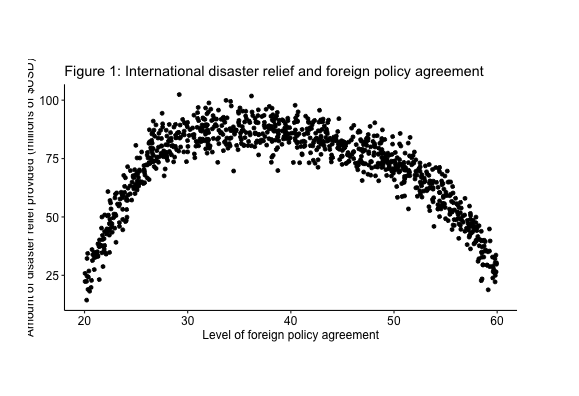
\includegraphics[width=0.9\textwidth]{q6.png}
		    \label{fig:pres_inc_prof}
	    \end{figure}

\clearpage


\end{document}
